% Don't modify this section unless you know what you're doing!
\documentclass[letterpaper,12pt]{article}
\usepackage{float}
\usepackage[spanish]{babel}
\selectlanguage{spanish}
\usepackage[utf8]{inputenc}
\usepackage{tabularx} % extra features for tabular environment
\usepackage{amsmath}  % improve math presentation
\usepackage{graphicx, wrapfig, subcaption, setspace, booktabs}
\usepackage{graphicx} % takes care of graphic including machinery

\usepackage[margin=1in,letterpaper]{geometry} % decreases margins
\usepackage{cite} % takes care of citations
\usepackage[final]{hyperref} % adds hyper links inside the generated pdf file
\usepackage{amsmath}
\usepackage{amssymb}
\usepackage{enumerate}
\usepackage{url}
\hypersetup{
	colorlinks=true,       % false: boxed links; true: colored links
	linkcolor=blue,        % color of internal links
	citecolor=blue,        % color of links to bibliography
	filecolor=magenta,     % color of file links
	urlcolor=blue         
}
%++++++++++++++++++++++++++++++++++++++++


\begin{document}

\title{Reporte de la Actividad 9}
\author{Daniela Olmos Velderrain\\Grupo 3}
\date{8 de mayo de 2019}

\maketitle

\section{Introducción}
El objetivo de esta actividad fue resolver numéricamente un sistema de ecuaciones diferenciales ordinarias que describe un sistema masa-resorte acoplado, representado en la siguiente figura:

\begin{figure}[H]
\centering
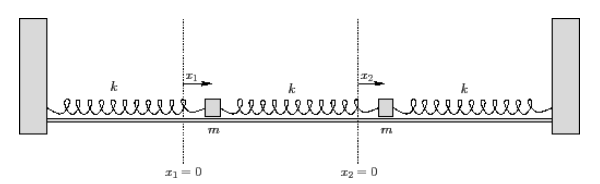
\includegraphics[width=0.4\textwidth]{esquema1.png}
\caption{\label{fig:graf1}: Sistema masa-resorte con dos grados de libertad. }
\end{figure}

En el presente reporte se describirá el procedimiento seguido para llegar a la solución del problema planteado, mostrando la teoría detrás del modelo físico, así como las consideraciones para llegar a una ecuación adecuada para trabajar en Python y la gráfica que muestra el resultado obtenido.



\section{Desarrollo}

\subsection{Marco teórico}
Un oscilador armónico es aquel sistema que cuando se deja en libertad fuera de su posición de equilibrio, vuelve hacia ella describiendo oscilaciones sinusoidales en torno a dicha posición estable. \\\\
Mediante la ley de Hooke, describimos la fuerza ejercida por un resorte sobre una masa como:
\[F=-kx\]

Donde $k$ es la constante elástica del resorte, $x$ es la distancia entre la posición de equilibrio y la masa, la cual denominamos como $m$.\\\\

De acuerdo a la segunda ley de Newton, sabemos que $F=ma=m\Ddot{x}$. Reemplazando la fuerza tenemos:
\[m\Ddot{x}=-kx\]

Si además tomamos en cuenta la fricción, esta ecuación resulta ser:
\[m\Ddot{x}=-kx-b\dot{x}\]
Donde b es el coeficiente de fricción.\\\\

El problema presentado en el esquema es un sistema de osciladores acoplados, ya que consta de varios osciladores individuales interconectados entre sí. 

\subsection{Metodología} 
Para encontrar la solución numérica del sistema de ecuaciones diferenciales, nos basamos en el algoritmo que aparece en el Cookbook de SciPy. Aquí se apoyan en las bibliotecas \emph{NumPy} y \emph{SciPy} para realizar los cálculos, empleando la función \emph{odeint}, la cual soluciona ecuaciones diferenciales de primer orden.\\\\
Sin embargo, el problema abordado aquí es distinto al nuestro, ya que en nuestro caso la configuración de masas y resortes incluye una pared y un resorte extra, como se muestra a continuación:

\begin{figure}[H]
\centering
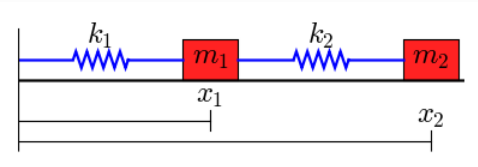
\includegraphics[width=0.4\textwidth]{esquema2.png}
\caption{\label{fig:graf1}: Sistema masa-resorte solucionado en el Cookbook de SciPy. }
\end{figure}

Las ecuaciones diferenciales que modelan este sistema son:

\begin{equation*}
    m_{1}\Ddot{x_{1}} + b_{1}\Dot{x_{1}} + k_{1}(x_{1} - L_{1}) - k_{2}(x_{2} - x_{1} - L_{2}) = 0 
\end{equation*}
\begin{equation*}
    m_{2}\Ddot{x_{2}} + b_{2}\Dot{x_{2}} + k_{2}(x_{2} - x_{1} - L_{2}) = 0  
\end{equation*} 

Además de las diferencias en el problema físico, el sistema de referencia tomado para las variables también resulta ser distinto, puesto que aquí se incluyen como parámetros las longitudes naturales de los resortes ($L_{1}$ y $L_{2}$), y las posiciones de las masas $x_{1}$ y $x_{2}$ se miden a partir de la pared izquierda, mientras que en primer sistema se mide el desplazamiento a partir de la posición de equilibrio para cada masa.\\\\

Basándonos en la solución propuesta en las notas de Richard Fitzpatrick, escribimos las ecuaciones de movimiento para las dos masas como:

\begin{equation*}
    m\Ddot{x_{1}} = - kx_{1} + k(x_{2} - x_{1})    
\end{equation*}
\begin{equation*}
    m\Ddot{x_{2}} = - k(x_{2} - x_{1}) + k(x_{2})    
\end{equation*}

Adaptando estas ecuaciones a nuestro nuevo sistema, tenemos:

\begin{equation}
    m_{1}\Ddot{x_{1}} = -b_{1}\Dot{x_{1}} + k_{1}(x_{1} - L_{1}) - k_{2}(x_{1} - L_{1} + L_{2} - x_{2}) 
\end{equation}
\begin{equation}
    m_{2}\Ddot{x_{2}} = -b_{2}\Dot{x_{2}} - k_{3}(x_{2} - L_{2}) - k_{2}(x_{2} - L_{2} + L_{1} - x_{1})  
\end{equation} 

Este es un par de ecuaciones diferenciales de segundo orden. Para resolverlas mediante la función de \emph{SciPy} debemos convertir esto en un sistema de primer orden, para ello introducimos las siguientes variables:

\[ y_{1} = \Dot{x_{1}} \]
\[ y_{2} = \Dot{x_{2}} \]

Reescribimos ahora las ecuaciones de segundo orden, obteniendo un sistema de cuatro ecuaciones de primer orden:

\[ \Dot{x_{1}} =  y_{1} \]

\begin{equation*}
    \Dot{y_{1}} = ( -b_{1}\Dot{y_{1}} + k_{1}(x_{1} - L_{1}) - k_{2}(x_{1} - L_{1} + L_{2} - x_{2}) ) / m_{1} 
\end{equation*}

\[ \Dot{x_{2}}  = y_{2} \]

\begin{equation*}
    \Dot{y_{2}} = (-b_{2}\Dot{y_{2}} - k_{3}(x_{2} - L_{2}) - k_{2}(x_{2} - L_{2} + L_{1} - x_{1}))/m_{2}  
\end{equation*} 

Estas son las ecuaciones que fueron implementadas en Python para ser resueltas mediante la función \emph{odeint}, generándose así un archivo de texto con las posiciones de las masas, las cuales fueron graficadas posteriormente.



\subsection{Resultados}
 Se tomaron las siguientes condiciones iniciales para el sistema:
 \[k_{1}=k_{2}=k_{3}=1\]
 \[m_{1}=m_{2}=1\] 
 \[L_{1}=L_{2}=1\]
 \[b_{1}=b_{2}=0\] 
 \[x_{1}=1, y_{1}=x_{2}=y_{2}=0\]
 
 Los parámetros para la gráfica fueron stoptime=30 y numpoints=750. El resultado fue el siguiente:

\begin{figure}[H]
\centering
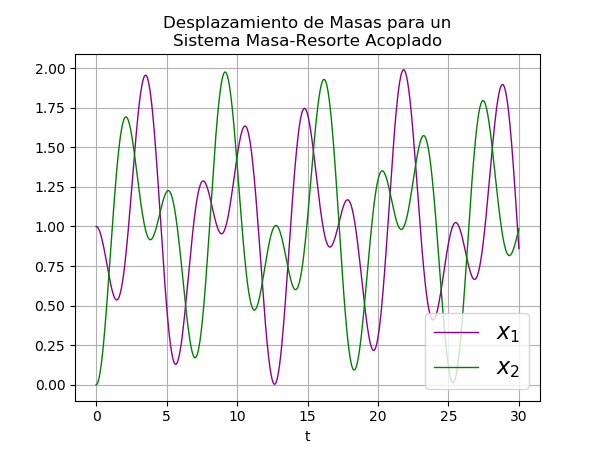
\includegraphics[width=0.5\textwidth]{dos_resortes.png}
\caption{\label{fig:graf1}: Sistema masa-resorte acoplado.}
\end{figure}


\section{Conclusiones}
Como pudimos apreciar, python puede ser una herramienta muy útil a la hora de modelar diversos sistemas físicos, ya que las librerías que contiene permiten trabajar en problemas matemáticos, como la resolución de ecuaciones diferenciales. \\\\
La mayor dificultad que presentó esta actividad fue el encontrar una ecuación adecuada para representar el comportamiento del fenómeno, ya que se debía modelar de acuerdo a un sistema de referencia adecuado para que el programa funcionara de manera correcta.\\\\

\section*{Bibliografía}
\begin{itemize}
\item \\Osciladores acoplados. Recuperado el 7 de mayo de 2019 desde \\https://es.wikipedia.org/wiki/Oscilador\_arm\%C3\%B3nico
\\

\item \\Osciladores acoplados. Recuperado el 7 de mayo de 2019 desde \\https://es.wikipedia.org/wiki/Osciladores\_acoplados
\\

\item \\Coupled spring-mass system. Recuperado el 7 de mayo de 2019 desde \\https://scipy-cookbook.readthedocs.io/items/CoupledSpringMassSystem.html
\\

\item \\Two Spring-Coupled Masses. Recuperado el 7 de mayo de 2019 desde \\https://farside.ph.utexas.edu/teaching/315/Waves/node18.html
\\

\end{itemize}

\end{document}
